\documentclass{article}
\usepackage[T1]{fontenc}
\usepackage{lmodern}
\usepackage{graphicx}
\usepackage{amsmath,amssymb}
\usepackage[a4paper,margin=2cm]{geometry}
\usepackage[absolute,overlay]{textpos}
\setlength{\TPHorizModule}{1mm}
\setlength{\TPVertModule}{1mm}
\usepackage[indonesian]{babel}
\usepackage{hyperref}
\setlength{\emergencystretch}{2em}
% unit: Halaman 17

\begin{document}

% === Halaman 17 (llm) ===

\vspace{214.73mm}

Run program

% deskripsi: Screenshot cuplikan kode Python yang mendemonstrasikan implementasi Caesar Cipher untuk enkripsi dan dekripsi pesan, lengkap dengan input pengguna dan output yang dihasilkan.
% bbox normalisasi: [0.0400, 0.1840, 0.9580, 0.9070]
\begin{textblock*}{192.78mm}(8.40mm,54.65mm)
\noindent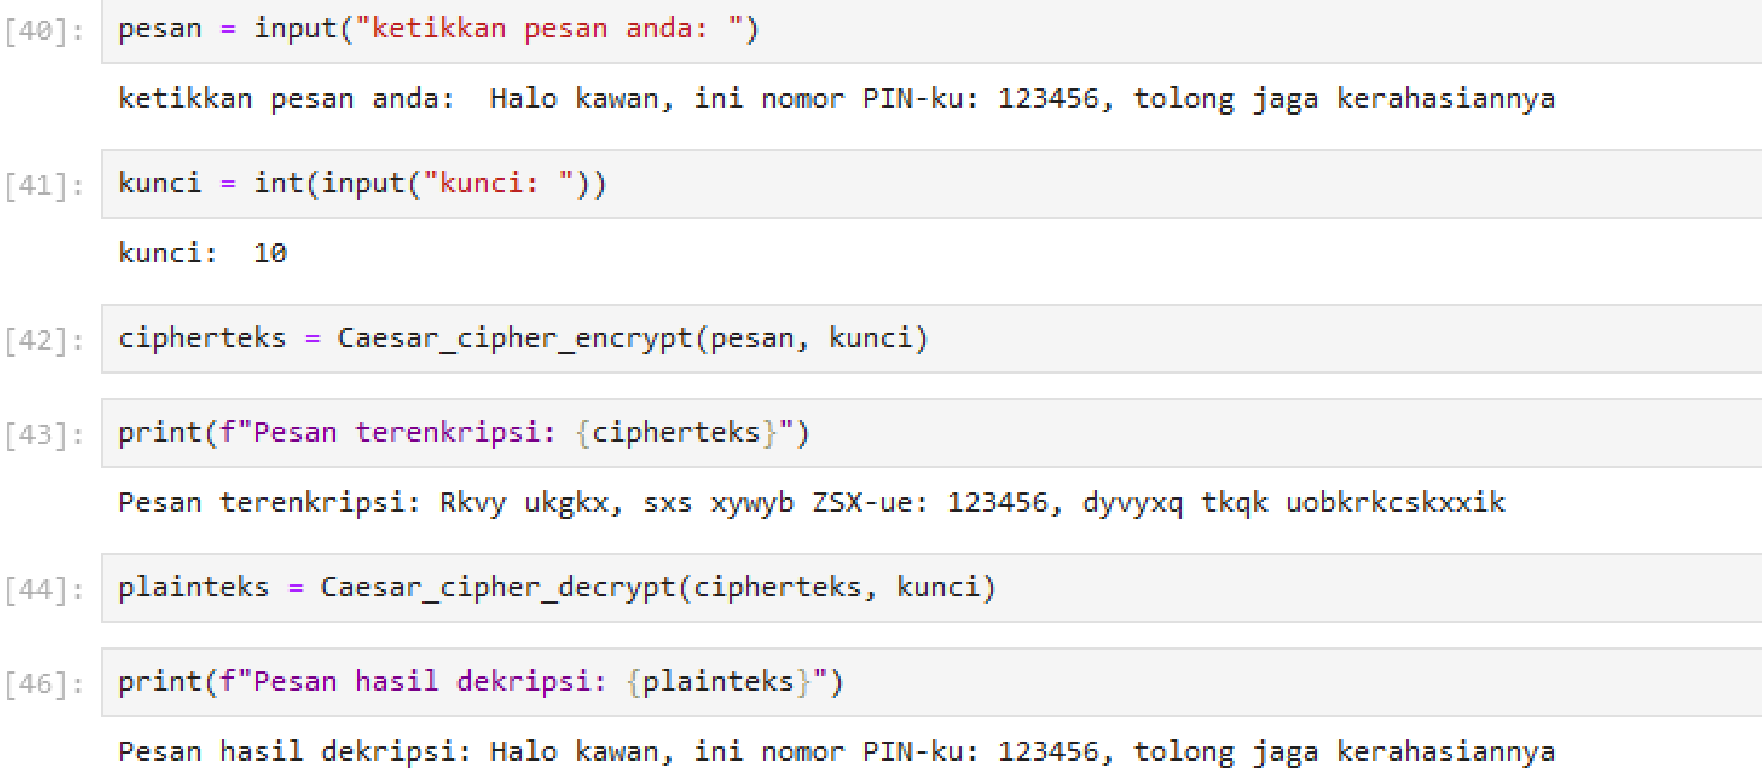
\includegraphics[width=192.78mm,height=214.73mm]{../../images/llm/page_017_img_01.png}%
\end{textblock*}

\end{document}
